\documentclass[11pt]{article}

% Robust arXiv-friendly workflow:
% - Engine: pdfLaTeX
% - Bibliography: BibTeX + natbib (numeric)
% - Fonts: default Latin Modern (clean math); optional Times-like via newtx

% Preamble for arxiv_robust (pdfLaTeX-first)

% ---- Encoding & fonts (MOST robust on arXiv) ----
\usepackage[T1]{fontenc}
\usepackage[utf8]{inputenc}

% Minimal Unicode support for text pasted/extracted from DOCX.
% Keep mappings conservative and math-safe.
\usepackage{newunicodechar}
\newunicodechar{′}{\ensuremath{^{\prime}}}
\newunicodechar{″}{\ensuremath{^{\prime\prime}}}
\newunicodechar{−}{\ensuremath{-}}
% Make dashes safe in math mode (prevents "\textendash invalid in math mode" warnings)
\providecommand{\UnicodeEnDash}{\ifmmode\text{--}\else\textendash\fi}
\providecommand{\UnicodeEmDash}{\ifmmode\text{---}\else\textemdash\fi}
\newunicodechar{–}{\UnicodeEnDash}
\newunicodechar{—}{\UnicodeEmDash}
\newunicodechar{≤}{\ensuremath{\le}}
\newunicodechar{≥}{\ensuremath{\ge}}
\newunicodechar{≈}{\ensuremath{\approx}}
\newunicodechar{∝}{\ensuremath{\propto}}
\newunicodechar{∈}{\ensuremath{\in}}
\newunicodechar{×}{\ensuremath{\times}}
\newunicodechar{·}{\ensuremath{\cdot}}
\newunicodechar{∇}{\ensuremath{\nabla}}
\newunicodechar{∂}{\ensuremath{\partial}}
\newunicodechar{⊙}{\ensuremath{\odot}}
\newunicodechar{☉}{\ensuremath{\odot}}
\newunicodechar{★}{\ensuremath{\star}}
\newunicodechar{☆}{\ensuremath{\star}}
\newunicodechar{□}{\ensuremath{\Box}}
\newunicodechar{■}{\ensuremath{\blacksquare}}
\newunicodechar{κ}{\ensuremath{\kappa}}
\newunicodechar{Λ}{\ensuremath{\Lambda}}
\newunicodechar{Δ}{\ensuremath{\Delta}}
\newunicodechar{Φ}{\ensuremath{\Phi}}
\newunicodechar{Ψ}{\ensuremath{\Psi}}
\newunicodechar{Ω}{\ensuremath{\Omega}}
\newunicodechar{Υ}{\ensuremath{\Upsilon}}
\newunicodechar{α}{\ensuremath{\alpha}}
\newunicodechar{β}{\ensuremath{\beta}}
\newunicodechar{γ}{\ensuremath{\gamma}}
\newunicodechar{δ}{\ensuremath{\delta}}
\newunicodechar{ε}{\ensuremath{\epsilon}}
\newunicodechar{η}{\ensuremath{\eta}}
\newunicodechar{λ}{\ensuremath{\lambda}}
\newunicodechar{μ}{\ensuremath{\mu}}
\newunicodechar{ν}{\ensuremath{\nu}}
\newunicodechar{π}{\ensuremath{\pi}}
\newunicodechar{ρ}{\ensuremath{\rho}}
\newunicodechar{σ}{\ensuremath{\sigma}}
\newunicodechar{τ}{\ensuremath{\tau}}
\newunicodechar{φ}{\ensuremath{\phi}}
\newunicodechar{χ}{\ensuremath{\chi}}
\newunicodechar{ψ}{\ensuremath{\psi}}
\newunicodechar{ω}{\ensuremath{\omega}}

% Default: Latin Modern (Computer Modern successor; excellent math coverage)
\usepackage{lmodern}

% Optional: Times-like text+math (common physics look)
% Enable by uncommenting BOTH lines below and commenting out lmodern above.
% \usepackage{newtxtext}
% \usepackage{newtxmath}

\usepackage[margin=1in]{geometry}
\usepackage{microtype}

% ---- Math ----
\usepackage{amsmath,amssymb}
\usepackage{mathtools}
\usepackage{bm}

% ---- Figures & tables ----
\usepackage{graphicx}
\usepackage{booktabs}
\usepackage{array}
\usepackage{longtable}

% ---- References (numeric) ----
\usepackage[numbers,sort&compress]{natbib}

% ---- Hyperlinks (keep conservative for arXiv) ----
\usepackage[hidelinks]{hyperref}

% Pandoc-ish compatibility helpers (harmless; useful if you paste content)
\providecommand{\tightlist}{%
  \setlength{\itemsep}{0pt}\setlength{\parskip}{0pt}}

% Project macros (keep minimal; arXiv-friendly)

% Common operators
\newcommand{\dd}{\mathrm{d}}
\newcommand{\ee}{\mathrm{e}}
\newcommand{\ii}{\mathrm{i}}

% Vectors/tensors (choose a convention and stick to it)
\newcommand{\vect}[1]{\boldsymbol{#1}}
\newcommand{\tensor}[1]{\mathbf{#1}}

% Derivatives
\newcommand{\pd}[2]{\frac{\partial #1}{\partial #2}}
\newcommand{\pdd}[2]{\frac{\partial^2 #1}{\partial #2^2}}
\newcommand{\od}[2]{\frac{\dd #1}{\dd #2}}
\newcommand{\odd}[2]{\frac{\dd^2 #1}{\dd #2^2}}


\title{Intrinsic Response Sector as Dark Gravity: A GR-Compatible Candidate Identity for the Cold Dark Matter Role (SPARC-175)}
\author{Robert D.\ Kitcey\\Independent Researcher\\\texttt{rkitcey@lernaean.net}}
\date{February 2026}

\begin{document}
\maketitle

% If a DOCX->LaTeX bootstrap exists, include it directly.
% This provides a complete, publishable draft while allowing incremental
% migration into the curated section files.
\IfFileExists{sections/99_pandoc_body.tex}{
	\input{sections/99_pandoc_body}
}{
	\begin{abstract}
	We present a falsification-first, galaxy-domain framework for explaining rotation-curve anomalies without assuming particulate cold dark matter. Working within standard general relativity (GR), we define a response-sector stress--energy $T^{\mathrm{resp}}_{\mu\nu}$ as the minimal effective source required so that the weak-field metric potentials inferred from kinematics satisfy the Einstein equation with baryons. This definition is ontologically agnostic and is best read as an EFT/constitutive-closure candidate. Observed rotation curves define a model-independent residual, which we compress with a one-parameter boundary-layer closure activated near a baryonic transition radius. Applied to 175 galaxies from the SPARC database, this model yields very strong improvement over a baryons-only model for 92\% of systems and passes a Bayesian Information Criterion (BIC) overfitting test in 97\% of cases. Crucially, we demonstrate that this 1-parameter response model is strongly preferred by BIC over standard 2-parameter NFW and Burkert dark matter halo models in over 90\% of the SPARC sample. Further, 5-fold cross-validation shows the response model has significantly lower out-of-sample prediction error (mean RMSE = 3.1 km/s) than the NFW model (mean RMSE = 4.9 km/s). The baryonic Tully--Fisher relation is recovered as an empirical consequence (Spearman $r_s = 0.95$). These results establish the response sector as a parsimonious and predictively powerful alternative to standard halo models for describing galactic dynamics.

\paragraph{Keywords.}
Galaxy rotation curves; dark matter alternatives; dark matter candidates; dark matter identity; general relativity; gravitation; effective field theory; response-sector stress--energy; boundary-layer physics; SPARC database; falsification criteria.

	\end{abstract}

	\section*{Executive Summary}

The dark-matter paradigm explains galactic rotation curve anomalies by postulating a new, non-luminous matter component. Despite decades of null results in direct, indirect, and collider searches, the hypothesis persists largely because no comparably rigorous alternative has been tested against the full breadth of observational data. This paper develops and tests such an alternative.

We keep the Einstein tensor standard (general relativity) and do not assume particulate cold dark matter (CDM). Instead, we use observed galactic phenomenology---rotation curves from the SPARC database of 175 galaxies---to infer the effective potentials and effective stress--energy required on the right-hand side of the Einstein equation, then compress that freedom with a low-degree-of-freedom ``intrinsic medium response'' closure.

The organizing principle is to treat the Einstein equation as an inverse problem,
\begin{equation}
G_{\mu\nu} = 8\pi G\left(T^{\mathrm{bar}}_{\mu\nu} + T^{\mathrm{resp}}_{\mu\nu}\right),
\end{equation}
where $T^{\mathrm{resp}}_{\mu\nu}$ is the response-sector stress--energy required by the observed phenomenology and then constrained by a low-degree-of-freedom closure.

\begin{itemize}
\item explains galaxy halo phenomenology without particulate CDM, and
\item admits a cosmological completion consistent with the empirical $\Lambda$CDM success set.
\end{itemize}

The response sector is activated near a baryonic boundary layer, produces an asymptotic tail in the extra acceleration, and is described by $\le 2$ degrees of freedom per galaxy. Across 175 SPARC galaxies, 92\% show very strong improvement over baryons-only, 97\% pass BIC overfitting tests, and the baryonic Tully--Fisher relation emerges as a consequence rather than an imposed prior.

We present explicit falsification criteria, discriminant tests (including lensing-facing statements and cosmological viability requirements), and a domain-partitioned roadmap from galaxy phenomenology through gravitational slip to large-scale structure. Claims are partitioned by domain: this work establishes the galaxy-domain closure and enumerates the cosmological completion requirements and discriminants.


	\tableofcontents

	% AUTO-GENERATED by scripts/generate_section_skeleton_from_outline.py
% Edit the individual section files; re-run generator only to add missing stubs.

\section{Introduction}

% Seeded from DOCX text extraction (see scratch/by_section/10_introduction.tex).
% TODO: Verify wording + fill in missing equations from the PDF.

For nearly a century, gravitational anomalies at galactic and cosmological scales have been parameterized by an additional non-luminous sector. The $\Lambda$CDM concordance model fits the CMB, BAO, and large-scale structure with high precision when cold dark matter (CDM) is treated as an effectively pressureless gravitating component.

Yet the microphysical identity of that dominant non-baryonic component remains empirically unresolved. Many canonical weak-scale interaction scenarios have been constrained by direct detection, indirect searches, and collider experiments. This motivates renewed attention to alternatives that treat the dark sector first as an empirical role and only secondarily as an ontological identity.

This paper develops an inverse-GR alternative consistent with the Discussion framing in \S9: we retain standard GR on the left-hand side and ask what effective stress--energy must appear on the right-hand side if we do not assume particulate CDM. The organizing equation is \emph{(see PDF)}, where \emph{(see PDF)} is defined as the effective response sector required by the observed phenomenology. This definition is ontologically agnostic; we do not claim spacetime is literally a fluid or solid, only that it admits an EFT/constitutive response closure.

In the circular-orbit regime, the data provide \emph{(see PDF)} and therefore \emph{(see PDF)}. The baryonic prediction \emph{(see PDF)} is assembled from SPARC's stellar and gas components with specified mass-to-light ratios. The model-independent residual \emph{(see PDF)} defines the ``missing curvature'' attributable in $\Lambda$CDM to a halo, and attributable here to the response sector.

The inverse mapping alone is underdetermined: many effective sources could reproduce a given \emph{(see PDF)}. The scientific content of this work is therefore compression. We impose a boundary-layer closure in which the response activates near a baryonic transition radius \emph{(see PDF)} (operationally where \emph{(see PDF)}) and satisfies an approximate flux-conservation law outside the activation zone, yielding an asymptotic \emph{(see PDF)} tail with $\le 2$ degrees of freedom per galaxy.

We further distinguish \emph{(see PDF)} (a global fit amplitude under the imposed closure) from \emph{(see PDF)} (a robust outer estimator computed directly from the outer \emph{(see PDF)} subset). Their strong agreement in rank across SPARC-175 supports the interpretation that the inferred response amplitude tracks genuine outer physics, while deviations diagnose where a single fixed shape requires extension.

Rotation curves primarily constrain the Newtonian-gauge potential \emph{(see PDF)}; lensing constrains the Weyl potential \emph{(see PDF)}. Consistent with \S9, we treat lensing as a gateway discriminant between Branch A (metric equivalence, \emph{(see PDF)}) and Branch B (slip-allowed, \emph{(see PDF)} localized to activation zones).

\begin{figure}[t]
	\centering
	% TODO: Add schematic figure file under figures/ and include it here.
	% \includegraphics[width=0.9\linewidth]{figures/figure1_concept.pdf}
	\caption{Conceptual schematic of the response-sector framework. The central luminous disk represents the baryonic mass distribution. Concentric lobes illustrate the radial residual $\Delta a$, with compression ($\Delta a > 0$, orange) and rarefaction ($\Delta a < 0$, blue) zones. The dashed ellipse marks the transition radius $R_t$ where \emph{(see PDF)}. Two amplitude estimators are distinguished: \emph{(see PDF)} (robust outer-subset Huber location) and \emph{(see PDF)} (single-parameter model-closure fit). The oscillatory structure is schematic; per-galaxy profiles (see \S6) need not exhibit clean alternation.}
	\label{fig:concept_schematic}
\end{figure}

We proceed as follows. Section 2 develops the inverse-GR construction from kinematics to effective stress--energy. Section 3 specifies the minimal response-sector closure. Sections 4--5 report results across 175 galaxies. Sections 6--8 state falsification criteria and the domain-partitioned validation ladder. Section 9 provides context (MOND/TeVeS, emergent/nonlocal gravity), strengths and limitations, and the role-versus-identity framing. Section 10 concludes.

\section{From Phenomenology to Effective Source: The Inverse-GR Construction}

% TODO: Port text/equations into each subsection; verify against the PDF.

The standard approach to galaxy dynamics begins with a theoretical mass model (baryons + dark matter) and predicts observable kinematics. We invert this logic: we begin with observed kinematics and infer what effective source is required within standard GR.

\subsection{Kinematics to Required Radial Acceleration}
For each galaxy in the SPARC database, the observed rotation curve provides the centripetal acceleration at galactocentric radius $R$:

\emph{(Equation from PDF: $a_{\mathrm{obs}}(R)$ in terms of $V(R)$ and $R$.)}

The baryonic prediction $a_{\mathrm{bar}}(R)$ is constructed from SPARC's decomposed photometric and gas-mass components \citep{Lelli2016SPARC}, with a chosen stellar mass-to-light ratio $\Upsilon_\star$. The residual defines the ``missing curvature'' in the circular-orbit sector:

\emph{(Equation from PDF: $\Delta a(R) \equiv a_{\mathrm{obs}}(R) - a_{\mathrm{bar}}(R)$.)}

This residual is model-independent: it is a direct comparison of observed kinematics with the baryonic gravitational prediction. In the CDM interpretation, $\Delta a$ is sourced by an additional mass component. In the response-sector interpretation, it is the effective geometric response of spacetime to the baryonic source.

\subsection{Weak-Field Metric Potentials}
In the Newtonian gauge for weak gravitational fields, the line element takes the form:

\emph{(Equation from PDF: weak-field metric with potentials $\Phi$ and $\Psi$.)}

To leading order for nonrelativistic motion, the radial acceleration is $a \approx -\nabla \Phi$. Gravitational lensing depends on the Weyl combination $\propto (\Phi + \Psi)/2$. Thus, rotation curves primarily constrain $\Phi$, while lensing constrains the combination $(\Phi + \Psi)$. A metric-equivalent response-sector claim is strongest if it produces $\Phi \approx \Psi$ in the relevant regime; if it predicts gravitational slip ($\Phi \neq \Psi$), that slip becomes a key discriminant (see \S\,8).

\subsection{Effective Enclosed Mass and Density}
For spherically symmetric intuition (useful even for disk galaxies), circular orbits obey $V^2/R = GM(<R)/R^2$. Given the observed rotation curve, we define an effective enclosed mass:

\emph{(Equation from PDF: $M_{\mathrm{eff}}(<R)$ in terms of $V(R)$.)}

Subtracting baryons yields an effective extra enclosed mass and, by differentiation, an effective extra density:

\emph{(Equations from PDF: $\Delta M(<R)$ and $\rho_{\mathrm{eff}}(R)$ / $\Delta\rho(R)$.)}

For a flat outer rotation curve ($V \to \mathrm{const}$), one obtains $M \propto R$ and $\rho \propto R^{-2}$---the classic isothermal halo profile. In the response-sector interpretation, this effective density is not a new matter species; it is the effective stress--energy of the spacetime response to baryonic structure.

\subsection{Effective Stress–Energy: What Is Being Added in GR}
In standard GR, the Einstein equation reads $G_{\mu\nu} = 8\pi G\,T_{\mu\nu}$. The entire program is to interpret an additional contribution $T^{(\mathrm{resp})}_{\mu\nu}$ as a polarization-like response of the gravitational sector, activated by baryonic structure (especially at boundary/transition regions), with a small parameter set and a universal functional form. This makes the ``extra'' empirically necessary but not an ad hoc per-galaxy function.

The response-sector stress--energy admits a standard fluid decomposition:

\emph{(Equation from PDF: $T^{(\mathrm{resp})}_{\mu\nu}$ decomposed into $\rho$, $p$, 4-velocity, and anisotropic stress $\pi_{\mu\nu}$.)}

where $\rho$ is the effective halo density in the inverse-GR sense, $p$ determines whether the sector is dust-like on large scales, and the anisotropic stress directly controls gravitational slip and lensing deviations.

\subsection{Conservation Constraint}
By the Bianchi identity, $\nabla^\mu G_{\mu\nu} = 0$. If baryons are minimally coupled and follow $\nabla^\mu T^{(\mathrm{bar})}_{\mu\nu} = 0$, then $\nabla^\mu T^{(\mathrm{resp})}_{\mu\nu}$ must hold independently. If exchange between sectors is allowed, this predicts a (possibly screened) fifth-force/equivalence-principle violation sector that must be stated explicitly. In this work, we assume independent conservation.

\section{Minimal Response-Sector Model Specification}

% TODO: Port text/equations into each subsection; verify against the PDF.

The inverse-GR construction of \S\,2 shows what effective source is required. This section specifies a minimal closure that compresses the inverse freedom to $\le 2$ degrees of freedom per galaxy.

\subsection{Design Principles}
A response-sector model is parsimonious only if it satisfies three conditions. First, low-DOF compression: across galaxies, the inferred response must be well described by a universal shape family with $\mathcal{O}(1)$ parameters, not a bespoke function. Second, baryonic activation: the response must be tied to a baryonic invariant (an edge/transition proxy), limiting per-galaxy freedom. Third, out-of-sample prediction: the edge-amplitude statistic should be predictable from internal observables better than from environment proxies under cross-validation.

\subsection{Auxiliary-Field Boundary-Layer Model}
We introduce an auxiliary scalar field coupled to baryons through the action:

\emph{(Equation from PDF: action defining auxiliary field and coupling.)}

The key operational constraints are:

\begin{itemize}
\item ties activation to a baryonic invariant (an edge/transition proxy such as \emph{(see PDF)} or a surface-density proxy), not to a per-galaxy hand-fit function;
\item the weak-field static equation for the auxiliary field reduces, outside the activation region, to an approximate flux-conservation law $\nabla\cdot \bm{J}=0$ with radial $J$ in disk symmetry, yielding an asymptotic \emph{(see PDF)} tail;
\item this preserves standard GR on the left-hand side while adding a tightly constrained response sector on the right.
\end{itemize}

\subsection{Operational Implementation}
In practice, the boundary-layer model defines a transition radius $R_t$---the galactocentric radius nearest to where \emph{(see PDF)} peaks. The model prediction for the total circular velocity is:

\emph{(Equation from PDF: $V_{\mathrm{model}}^2(R)$ in terms of $V_{\mathrm{bar}}^2(R)$ and response contribution.)}

where \emph{(see PDF)} is the single amplitude parameter (in $\mathrm{km}^2\,\mathrm{s}^{-2}$) controlling the strength of the response, and \emph{(see PDF)} encodes the boundary-layer shape: zero for $R < R_t$, rising to an asymptotic tail for $R > R_t$. The fit minimizes the weighted residual against the observed rotation curve to determine the amplitude parameter for each galaxy.

\subsection{The Constitutive “Gravitational Dielectric” Alternative}
An equivalent weak-field formulation defines an effective polarization field $\bm{P}$ such that the modified Poisson equation becomes a constitutive law:

\emph{(Equation from PDF: modified Poisson/constitutive law with $\bm{P}$.)}

Then \emph{(see PDF)} plays the role of the effective response density. This formulation restricts $\bm{P}$ to depend on baryonic invariants and a small number of constants, and is embeddable in a covariant action for lensing and cosmological extensions.

\subsection{Three Completion Routes}
The response-sector bookkeeping is compatible with at least three microphysical completions:

\begin{itemize}
\item extra field/medium: $T^{(\mathrm{resp})}_{\mu\nu}$ arises from some field(s) \emph{(see PDF)};
\item modified gravity rewritten as effective source: higher-curvature or nonlocal terms moved to the right-hand side;
\item constitutive closure: \emph{(see PDF)}.
\end{itemize}

This paper establishes the galaxy-domain phenomenology without committing to a specific completion; the choice constrains lensing and cosmological predictions (see \S\,8).

\section{Data and Pipeline}

% TODO: Port text/equations into each subsection; verify against the PDF.

\subsection{The SPARC Database}
The Spitzer Photometry and Accurate Rotation Curves (SPARC) database \citep{Lelli2016SPARC} provides uniformly measured HI/H$\alpha$ rotation curves and $3.6\,\mu\mathrm{m}$ Spitzer photometry for 175 nearby galaxies spanning a factor of $\sim 10^4$ in luminosity, $\sim 10^2$ in size, and a wide range of morphologies (from gas-rich dwarfs to massive spirals). Each galaxy entry includes the observed circular velocity \emph{(see PDF: $V_{\mathrm{obs}}(R)$ with uncertainties)}, the baryonic rotation-curve components (stellar disk, gas, and where relevant, stellar bulge), the adopted distance and inclination, and data quality flags.

\subsection{Baryonic Velocity Construction}
The baryonic velocity prediction is assembled from SPARC components:

\emph{(Equation from PDF: $V_{\mathrm{bar}}^2 = V_{\mathrm{gas}}^2 + \Upsilon_{\star,\mathrm{disk}} V_{\mathrm{disk}}^2 + \Upsilon_{\star,\mathrm{bulge}} V_{\mathrm{bulge}}^2$ or equivalent.)}

where $\Upsilon_{\star,\mathrm{disk}}$ and $\Upsilon_{\star,\mathrm{bulge}}$ are the stellar mass-to-light ratios. We adopt \emph{(see PDF: baseline $\Upsilon_\star$ choice)} as the baseline, consistent with stellar population synthesis models at $3.6\,\mu\mathrm{m}$ \citep{McGaughSchombert2014}, with sensitivity sweeps across \emph{(see PDF: range of $\Upsilon_\star$)} to quantify photometric systematic uncertainties.

\subsection{Transition Radius Determination}
For each galaxy, we identify the transition radius $R_t$ as the measured radius closest to where \emph{(see PDF: baryonic/observed relation criterion)} crosses the empirical acceleration scale \emph{(see PDF: $a_0$ or equivalent)}. This is a data-derived quantity, not a free parameter.

\subsection{Fit Procedure and Amplitude Determination}
The single free parameter \emph{(see PDF: amplitude parameter, e.g. $Q$)} is determined for each galaxy by minimizing the weighted \emph{(see PDF: $\chi^2$ definition)} between \emph{(see PDF: model prediction)} and \emph{(see PDF: observed rotation curve)}. As an independent check, we compute \emph{(see PDF: robust outer amplitude estimator, e.g. $Q_{\mathrm{est}}$)}, a robust outer-subset estimator using Huber's M-estimator applied to the velocity deficit \emph{(see PDF: $\Delta V^2(R)$)} in the outer region ($R > R_t$). The Huber estimator down-weights outliers while remaining efficient under Gaussian conditions, providing an amplitude estimate that does not depend on the model's functional form.

\subsection{Six-Panel Diagnostic Atlas}
For each galaxy, a standardized six-panel diagnostic is produced:

\begin{enumerate}
\item rotation curve with \emph{(see PDF: $V_{\mathrm{obs}}$, $V_{\mathrm{bar}}$, and model curves)};
\item effective potential \emph{(see PDF: $\Phi(R)$ proxy)} vs. \emph{(see PDF: radius/acceleration)};
\item dyed spacetime potential-depth map (a visualization proxy, not a GR embedding);
\item 3D potential surface;
\item illustrative orbit diagram; and
\item residuals comparing both model closures against the raw baryonic deficit.
\end{enumerate}

This atlas serves as a comprehensive per-galaxy audit trail.

\section{Results Across 175 SPARC Galaxies}

% TODO: Port text/equations into each subsection; verify against the PDF.

\subsection{Global Fit Performance}
The boundary-layer response model with a single amplitude parameter \emph{(see PDF: $Q$)} provides substantial improvement over the baryons-only prediction across the SPARC sample. Using a \emph{(see PDF: $\chi^2$-based improvement metric)}, we find that the response-sector closure delivers strong improvements for the large majority of galaxies while remaining parsimonious (one fitted amplitude plus a data-derived transition radius).

\emph{(Table from PDF: global fit performance summary across 175 galaxies.)}

\subsection{Representative Galaxy Diagnostics}
To illustrate performance across the galaxy mass spectrum, we report representative six-panel diagnostics spanning gas-dominated dwarfs to massive spirals. The figures will be inserted during the PDF-faithful port (see PDF for current canonical visuals).

Representative cases discussed in the source draft include:
\begin{itemize}
\item NGC 2403 (intermediate-mass spiral);
\item DDO 154 (gas-dominated dwarf irregular);
\item NGC 2841 (massive high-surface-brightness spiral);
\item UGC 06614 (low-surface-brightness system).
\end{itemize}

\emph{(Figures from PDF: six-panel diagnostics for these galaxies.)}

\subsection{Emergent Baryonic Tully–Fisher Relation}
A critical test of any dark-matter alternative is whether it recovers the baryonic Tully--Fisher relation (BTFR): the tight empirical correlation between baryonic mass and asymptotic rotation velocity \citep{McGaugh2000}. In our framework, the BTFR is not imposed as a prior but emerges as a consequence of the boundary-layer closure.

\emph{(See PDF: correlation statement between fitted amplitude and BTFR proxy, with Spearman $\rho$ and $p$-value.)}

\subsection{Fitted vs. Robust Amplitude Comparison}
A key robustness check compares the model-fitted amplitude \emph{(see PDF: $Q_{\mathrm{fit}}$)} (from global minimization) with the independently computed \emph{(see PDF: $Q_{\mathrm{est}}$)} (from Huber robust estimation on the outer velocity deficit). Across 175 galaxies, the rank correlation is strong, supporting the claim that the fitted amplitude reflects outer-region physics rather than overfitting to inner structure.

\emph{(See PDF: Spearman $\rho$, fraction with $Q_{\mathrm{est}}/Q_{\mathrm{fit}} < 1$, and median ratio.)}

\subsection{Mass-to-Light Ratio Sensitivity}
Sweeping $\Upsilon_\star$ across \emph{(see PDF: the tested grid)} demonstrates that response-sector inferences are robust to plausible photometric systematics. While individual galaxy amplitudes shift with $\Upsilon_\star$, the global performance metrics and BTFR scaling remain stable.

\emph{(See PDF: median fractional change in amplitude across the $\Upsilon_\star$ sweep and the dynamic range of $Q$.)}

\subsection{Oscillatory Signatures and Negative-Q Galaxies}
Two galaxies \emph{(see PDF: named cases)} exhibit negative \emph{(see PDF: $Q$)} values---cases where the observed velocity falls below the baryonic prediction in the outer regions. Within the response-sector framework, these are interpreted as rarefaction-phase sampling of an oscillatory boundary-layer response: the response includes both compression ($\Delta a > 0$) and rarefaction ($\Delta a < 0$) phases, and some galaxies' observed radial coverage samples primarily the rarefaction phase.

More broadly, \emph{(see PDF: count and percentage)} of galaxies show at least one sign change in their velocity-deficit profiles. The characteristic oscillation wavelength scales with galaxy size (median \emph{(see PDF)}), consistent with standing-wave configurations in the scalar sector of the metric field that are distinct from transverse spin-2 gravitational waves.

\section{Empirical Validation Ladder}

Robust empirical claims require more than curve-fitting. This section defines the validation hierarchy that the response-sector framework must satisfy.

\subsection{Step 1: Data Reproducibility}

All results are generated from a single reproducible pipeline operating on the public SPARC database files. Inclusion criteria, missing-data handling, and quality flags are defined explicitly. The per-galaxy fitted summaries, six-panel diagnostics, and analysis tables are regenerated from a single command.

\subsection{Step 2: Baseline Fits and Residual Definitions}

The primary edge-amplitude measure is \textbf{(see PDF for definition; symbol and equation not recovered from DOCX extraction)}. Sensitivity alternates include \textbf{(see PDF for the ``Huber robust outer-subset'' definition)} and \textbf{(see PDF for the asymptotic-velocity-excess definition)}. Baseline scale controls include \textbf{(see PDF; list of baseline controls not recovered)} with distance \textbf{(see PDF; distance variable definition)} as an optional confounder check.

\subsection{Step 3: Non-Fragile Inference}

Rather than relying on asymptotic $p$-values, we employ permutation-based inference: two-tailed permutation $p$-values for Pearson and Spearman correlations, with a partial-correlation mode (residualizing both dependent and independent variables on controls). This is robust to non-normality, outliers, and small-sample effects.

\subsection{Step 4: Stratified Permutation Stress Tests}

To guard against confounding, we stratify permutation tests by:
\begin{itemize}
	\item SPARC quality flag \textbf{(see PDF; flag name/values not recovered)};
	\item distance quantiles;
	\item \textbf{(see PDF; additional stratification axis not recovered)} $\times$ distance quantiles; and
	\item coarse morphological type.
\end{itemize}
Any claimed correlation must survive all stratified tests to be considered robust.

\subsection{Step 5: Out-of-Sample Cross-Validation}

The decisive test uses repeated $k$-fold cross-validation to compare nested models: baseline (scale controls only), extended (scale + intrinsic-structure features), and full (scale + structure + environment). If the response-sector hypothesis is correct, intrinsic-structure features should improve out-of-sample prediction of the edge amplitude more than environment features.

\subsection{Step 6: Negative Controls}

Shuffled-environment columns should produce no significant correlations. Distance-only models serve as confounder detectors. These controls ensure that claimed signals are not artifacts of data structure.

\section{Falsification Criteria and Discriminant Tests}

A theory that cannot be falsified provides no scientific content. We state four explicit conditions under which the response-sector framework would be refuted.

\subsection{Criterion 1: Compression Failure}

If \textbf{(see PDF; target function/observable not recovered from DOCX extraction)} cannot be summarized by a universal low-DOF shape/amplitude tied to baryonic structure---if it requires an essentially free function per galaxy---then the ``materials reverse engineering'' story collapses into ad hoc curve-fitting and the framework is falsified as a parsimonious alternative.

\textbf{Status (DOCX-extracted; verify against PDF):} The single-parameter model achieves very strong improvement for 92\% of galaxies and passes BIC for 97\%, indicating compression holds across the SPARC sample.

\subsection{Criterion 2: Out-of-Sample Prediction Failure}

If internal predictors (baryonic structure, gas fraction, surface density) do not improve prediction of the edge amplitude in cross-validation beyond scale controls, the ``intrinsic boundary-layer'' causal story is not supported by the data.

\subsection{Criterion 3: Gravitational Slip / Lensing Inconsistency}

If the inferred extra potential needed for dynamics implies a (\textbf{see PDF; metric-potential pair not recovered}) pair that cannot match gravitational lensing constraints without adding new freedom, the metric-equivalence claim must be weakened or the framework revised. Specifically: if galaxy--galaxy lensing measurements require a different amplitude or profile than predicted by the response sector assuming \textbf{(see PDF; lensing/dynamics identification assumption)}, the model faces a decisive test (\S8).

\subsection{Criterion 4: Cosmological Growth Incompatibility}

If the response sector, extended to cosmological scales, produces a growth rate or perturbation structure that is incompatible with observed large-scale structure and CMB constraints, the framework cannot serve as a $\Lambda$CDM alternative (it may still be valid as a galaxy-domain model, but the ``go big'' program would be falsified).

\subsection{The Discriminant Triad}

If the framework is to serve as a serious $\Lambda$CDM-alternative candidate, three discriminant tests are paramount:
\begin{itemize}
	\item \textbf{Low-DOF compression across SPARC:} The response sector in the galaxy quasi-static limit is described by a universal family with \textbf{(see PDF; number of DOF per galaxy)} degrees of freedom per galaxy. Killer failure mode: needing an arbitrary function per galaxy.
	\item \textbf{Rotation vs.
	lensing consistency:} The response sector must give a definite relation between dynamics (\textbf{see PDF; rotation-curve observable}) and lensing (\textbf{see PDF; lensing observable}). If \textbf{(see PDF; no-slip condition)} in the relevant regime, state ``metric-equivalent in that regime.'' If not, predict where slip appears.
	\item \textbf{Cosmological growth and background viability:} Match background distances to first order and demonstrate that the response sector can cluster appropriately.
\end{itemize}

\section{Lensing and Cosmological Viability}

The galaxy-domain results of \S\S4--6 establish that the response sector works empirically for rotation curves. A credible $\Lambda$CDM-alternative candidate must additionally address lensing and cosmology. This section provides the first lensing-facing statement and the minimal cosmological viability sketch.

\subsection{Lensing: The Weyl Potential Constraint}

\begin{sloppypar}
Galaxy--galaxy lensing and cluster lensing constrain the Weyl potential \textbf{(see PDF; symbol/definition not recovered from DOCX extraction)}. In standard GR with a perfect-fluid source (including CDM), the gravitational slip
\textbf{(see PDF; slip definition not recovered)}
at leading order in the quasi-static weak-field limit. The response-sector framework must make a definite prediction for $\eta$.
\end{sloppypar}

\subsubsection{Working Hypothesis: Metric Equivalence}

As a first working hypothesis, we assume the response sector produces \textbf{(see PDF; ``zero slip'' condition not recovered)} (zero slip) in the galaxy quasi-static regime. This is the most $\Lambda$CDM-like option and the easiest to test: it predicts that the lensing mass inferred from the response-sector's rotation-curve fit matches the lensing mass measured directly. Specifically, the implied convergence $\kappa(R)$ can be computed from the fitted potential and compared against weak-lensing measurements.

\subsubsection{Gravitational Slip as a Discriminant}

If the response sector includes anisotropic stress \textbf{(see PDF; symbol/definition not recovered)}, it generically produces gravitational slip \textbf{(see PDF; symbol/definition not recovered)}. This would be a distinctive observational signature. We do not introduce a free slip function; rather, we note that the choice of microphysical completion (\S3.5) determines the slip prediction. If future lensing data require slip, this constrains the completion; if they exclude it, the completion must produce \textbf{(see PDF; no-slip condition)}.

\subsection{Cosmological Background}

For the response sector to serve as a CDM replacement on cosmological scales, its effective energy density must evolve approximately as \textbf{(see PDF; scaling not recovered)} (dust-like) over the redshift range relevant for structure formation and distance measurements. This is the background viability requirement: the response sector must not ruin the distance--redshift relation that $\Lambda$CDM fits well.

\subsection{Cosmological Perturbations}

At the perturbation level, the response sector must cluster appropriately to produce the observed matter power spectrum and CMB angular power spectrum. A dust-like clustering component with an effective sound speed close to zero \textbf{(see PDF; symbol/definition not recovered)} over the relevant scales would most closely mimic CDM perturbations. If the response sector introduces a significant effective sound speed or anisotropic stress at cosmological scales, it will modify the growth rate and ISW effect in potentially detectable ways.

\subsection{Domain Partition and Honest Scope}

We adopt explicit domain partitioning: this work establishes the galaxy-domain closure and demonstrates empirical viability at rotation-curve scales. The lensing and cosmological domains are enumerated as defined requirements, not claimed results. The language discipline is: ``This work establishes the galaxy-domain closure and enumerates the cosmological completion requirements and discriminants.''

\section{Discussion}

\subsection*{Note on citations}
Bracket-number citations from the donor extraction have been converted to \texttt{natbib} citations where possible.

\subsection{The Response Sector}

\textbf{(see PDF; response-sector symbol not recovered from DOCX extraction)} is the effective stress--energy required so that the metric (or potentials) inferred from galaxy phenomenology satisfies the Einstein equation with baryons. This definition is ontologically agnostic---it does not commit to a microscopic composition of spacetime. We avoid claiming spacetime ``is literally'' a fluid or solid; instead, we describe the framework as an EFT/constitutive closure candidate.

\subsection{Relation to MOND and TeVeS}

Modified Newtonian Dynamics (MOND) \citep{Milgrom1983} shares the empirical acceleration scale $a_0$ and produces flat rotation curves through a modified force law. The response-sector framework differs in several respects: it retains standard GR on the left-hand side (the geometry is not modified); it provides an explicit stress--energy interpretation; it naturally accommodates both compression and rarefaction phases; and it admits a cosmological completion route. MOND's relativistic extension TeVeS \citep{Bekenstein2004} introduces a scalar and vector field---one of our completion routes (\S3.5i) is structurally similar but derived from an inverse-GR starting point rather than a modified-gravity one.

\subsection{Relation to Emergent Gravity and Nonlocal Gravity}

Verlinde's emergent gravity program \citep{Verlinde2017} derives a MOND-like force from entropic considerations. The response-sector approach is compatible but more conservative: we do not assume a thermodynamic origin for gravity, only that the gravitational sector admits an effective constitutive response. Nonlocal gravity models \citep{DeserWoodard2007} can be rewritten as effective sources on the right-hand side of the Einstein equation, placing them within our bookkeeping framework.

\subsection{Strengths of the Current Work}

The primary contributions of this paper are:
\begin{itemize}
	\item a mathematical framework (inverse-GR $\to$ response-sector closure) that makes the ``alternative to CDM'' concept precise within standard GR;
	\item systematic testing against 175 galaxies spanning \textasciitilde{}$10^4$ in luminosity;
	\item independent confirmation of fitted amplitudes by a robust estimator;
	\item explicit falsification criteria stated in advance; and
	\item a domain-partitioned roadmap that acknowledges what is and is not claimed.
\end{itemize}

\subsection{Limitations and Open Questions}

The framework as presented has clear limitations. The boundary-layer model is phenomenological: the precise form of \textbf{(see PDF; boundary-layer functions not recovered)} and \textbf{(see PDF; boundary-layer functions not recovered)} is not derived from first principles. The lensing prediction is a working hypothesis, not a tested result. Cosmological viability is stated as a requirement, not demonstrated. Galaxy clusters---where the CDM paradigm is well-tested---are not addressed. Pressure-supported systems (elliptical galaxies, galaxy groups) require extension beyond the circular-orbit framework. These limitations define the research program going forward.

\subsection{The Historical Lesson}

The Vulcan episode provides a cautionary tale: gravitational anomalies initially attributed to unseen matter ultimately revealed deeper geometric structure. We do not claim the contemporary analogy is exact---the dark-matter hypothesis is vastly more successful and well-motivated than Vulcan ever was---but the structural lesson remains: when a gravitational anomaly is observed, both matter-based and geometry-based explanations deserve rigorous investigation. The persistent null results in dark-matter searches lend urgency to this investigation.

\subsection{A Candidate Identity for the Cold Dark Matter Role}

\subsubsection{Role vs. Identity: A Formal Distinction}

The Lambda Cold Dark Matter ($\Lambda$CDM) model stands as the standard paradigm of cosmology, a testament to its success in explaining phenomena from the Cosmic Microwave Background (CMB) to large-scale structure \citep{Planck2018VI2020}. Yet, as Kuhn argued, the accumulation of significant anomalies is the necessary precondition for scientific revolution \citep{Kuhn1962}. For $\Lambda$CDM, the central anomaly is existential: after decades of engagement, every attempt to directly identify the foundational particle of cold dark matter has returned a null result \citep{UndagoitiaRauch2016,LZ2023}.

This motivates a formal distinction between the role of dark matter and its identity. This distinction is critical for a productive scientific dialogue.

\subsection{Defining the CDM Role}

In the language of General Relativity (GR), the CDM role is the assertion that there exists an effective stress-energy tensor sector, \textbf{(see PDF; CDM-role sector symbol not recovered)}, such that the Einstein Field Equations are satisfied:

\textbf{(see PDF; Einstein-equation display equation not recovered from DOCX extraction)}

This combined tensor must yield a metric that reproduces the full suite of geodesic phenomenology: time-like geodesics (galaxy and cluster dynamics), null geodesics (gravitational lensing), and cosmological perturbations (structure growth and the CMB power spectrum) \citep{Planck2018VI2020}. The minimal constraints on this role are that the total stress-energy is conserved \textbf{(see PDF; conservation equation not recovered)} and that the resulting phenomenology is consistent across all observational domains.

\subsection{The Intrinsic Response as a Candidate Identity}

The intrinsic response framework proposes a specific identity to fill this role. It posits that the extra sector is not an independent entity with its own initial conditions (i.e., a particle fluid), but is instead a constitutive response functional of the baryonic sector itself:

\textbf{(see PDF; constitutive-response equation not recovered from DOCX extraction)}

This claim is profound: it suggests the gravitational phenomenon of dark matter is real, but it is an emergent, structured response of the spacetime metric to baryonic matter. The ``darkness'' is simply that this response is non-luminous and need not have electromagnetic couplings. This reframes the 50-year null detection record not as a failure to find dark matter, but as a stunning success in defining what it is not: a particle with non-gravitational interactions. Intrinsic response arguably elegantly fits both these ``nots'' as well as the phenomenology. The null results have carved out a residual space of possibility shaped exactly like a geometric, field-theoretic response---a puzzle piece for which the intrinsic response is a precise fit.

This is not a competitor to dark matter; it is a candidate for its identity. It avoids the primary vulnerability of Modified Newtonian Dynamics (MOND) and its relativistic extensions like TeVeS, which must explain away the evidence for a dark component on cluster and cosmological scales \citep{Milgrom1983,Bekenstein2004}. Instead, it seeks to be that component.

\subsubsection{A Falsifiable Validation Plan: The Discriminants Ladder}

A candidate identity warrants engagement only if it is falsifiable. The intrinsic response framework offers a clear validation plan in the form of a ``discriminants ladder,'' where each rung represents a decisive empirical test. A crucial first step is to declare a default theoretical branch for the galaxy regime:
\begin{itemize}
	\item \textbf{Branch A (Metric-Equivalent):} The scalar potentials are equal \textbf{(see PDF; condition not recovered)}, implying no gravitational slip. Lensing follows dynamics in the standard way.
	\item \textbf{Branch B (Slip-Allowed):} The potentials differ \textbf{(see PDF; condition not recovered)} in the boundary-layer regions, predicting a specific lensing-dynamics mismatch.
\end{itemize}

\subsubsection{Development Gateway: Branch Selection as an Explicit Research Fork}

The framework does not treat Branch A vs.
Branch B as a philosophical preference; it treats this as a development gateway that future work must adjudicate empirically.

If Branch A (metric-equivalent, \textbf{see PDF; no-slip condition}) holds in the galaxy regime: then lensing is a cross-check of the same metric potential inferred from dynamics, and the response sector behaves as a metric-equivalent ``dark gravity'' identity.

If Branch B (slip-allowed, \textbf{see PDF; slip condition} in boundary layers) is supported by data: then the response sector predicts a controlled, baryon-conditioned mismatch between dynamical and lensing inferences, providing a sharper discriminant and a tighter handle on covariant completion.

In both cases, failure occurs only if the required behavior cannot be achieved without reintroducing an independent, freely specified pressureless dark fluid (i.e., restoring the same degrees of freedom intrinsic response is meant to compress).

This ladder provides a clear, pre-registered path to validation or falsification, moving the debate from philosophical preference to empirical adjudication.

Adopting Branch A as the default, the ladder of falsifiers is as follows:

\textbf{(see PDF; Table 2 ``Rung Table (Branch A)'' not recovered from DOCX extraction)}

Branch B (Slip-Allowed): We allow a localized gravitational slip,
\textbf{(see PDF; slip functional form not recovered)}
in boundary/activation regions (e.g., near \textbf{see PDF; transition radius symbol}, within width \textbf{see PDF; width symbol}), while recovering \textbf{(see PDF; recovery condition)} in regimes where GR is tightly tested (Solar System) and/or where the response is inactive.

Adopting Branch B as the default, the ladder of falsifiers is as follows:

\textbf{(see PDF; Table 3 ``Rung Table (Branch B)'' not recovered from DOCX extraction)}

Branch B note: In this branch, weak and strong lensing are not expected to be identical to a metric-equivalent mapping from rotation curves; instead, lensing becomes the primary probe of slip structure and its activation rules.

\subsubsection{From Critique to Collaboration: A Playbook for Scientific Engagement}

The framework's incomplete status is not a vulnerability but a well-defined research opportunity, characteristic of a progressive research program in the sense of Lakatos \citep{Lakatos1978}. It invites collaboration by turning common criticisms into testable questions, as summarized in the following playbook:

\textbf{(see PDF; Table 4 ``Criticism and Rebuttal'' not recovered from DOCX extraction)}

\subsubsection{Conclusion: The Case for Engagement}

The intrinsic response framework offers a compelling synthesis in the long-standing dark matter debate. It reframes the problem by proposing a candidate identity---an emergent metric response---that is shaped by the very null results that have placed the particle hypothesis under strain. It is ontologically parsimonious, empirically grounded in the tight kinematic correlations of galaxies \citep{McGaughLelliSchombert2016}, and structured as a progressive and falsifiable research program.

The framework is incomplete, but it is not vague. It has moved beyond speculation to make specific, testable predictions that distinguish it from both standard $\Lambda$CDM and MOND-like alternatives \citep{BullockBoylanKolchin2017,Verlinde2017}. For these reasons, it has earned the right to serious scientific engagement. The question is no longer whether it is too incomplete to consider, but whether it is too compelling to ignore.



\section{Conclusion}

We presented a falsification-first, galaxy-domain response-sector framework that makes an ``alternative to particulate CDM'' precise within standard GR. The response sector \textbf{(see PDF; response-sector symbol not recovered from DOCX extraction)} is defined as the effective stress--energy required so that the metric potentials inferred from galaxy phenomenology satisfy \textbf{(see PDF; Einstein equation not recovered from DOCX extraction)} with baryons fixed by SPARC mass models. As emphasized in \S9, this definition is ontologically agnostic and is best read as an EFT/constitutive-closure candidate rather than a literal mechanical medium.

Using SPARC-175, we showed that a low-DOF boundary-layer closure producing an asymptotic \textbf{(see PDF; tail notation not recovered)} tail yields strong improvement over baryons-only fits across the sample and recovers the BTFR as an empirical consequence. Robustness is strengthened by separating \textbf{(see PDF; model-fitted amplitude symbol not recovered)} from a model-free outer estimator \textbf{(see PDF; outer estimator symbol not recovered)}; their strong agreement in rank supports that the inferred amplitude is not an artifact of inner weighting, while discrepancies diagnose inner--outer shape tension and motivate minimal extension (e.g., a width parameter).

The work is deliberately scoped. Several limitations stated in \S9 remain open: the activation/closure is phenomenological rather than first-principles; lensing consistency is a working hypothesis pending measurement; clusters and pressure-supported systems require extension; and cosmological viability is an explicit requirement rather than a demonstrated result. These are not rhetorical caveats but the defined research program.

Accordingly, we pre-register a validation ladder:
\begin{itemize}
	\item continued compression and cross-validation on rotation curves;
	\item lensing adjudication of Branch A (\textbf{see PDF; metric-equivalent condition}) versus Branch B (slip-allowed, \textbf{see PDF; slip condition} in activation zones);
	\item cluster-regime scaling tests; and
	\item perturbation-level cosmological consistency.
\end{itemize}


\appendix

\section{Appendix A: Comprehensive Symbol Glossary}

This appendix is intended to provide a comprehensive glossary of symbols used throughout the paper.

\textbf{(see PDF; Table 5 ``Comprehensive Symbol Glossary'' not recovered from DOCX extraction)}

\noindent The glossary table is organized with the following columns:
\begin{itemize}
	\item Symbol (as written in text)
	\item Mathematical notation
	\item Definition
	\item Units
	\item Notes / context within the framework
\end{itemize}

\noindent \textbf{Unit conventions (as stated in donor extraction; verify against PDF):} $R$ in kpc; velocities in km/s; accelerations in $(\mathrm{km/s})^2/\mathrm{kpc}$. Conversion: $1\, (\mathrm{km/s})^2/\mathrm{kpc} = 10^6/\texttt{kpc\_in\_m}\,\mathrm{m/s^2}$, with \texttt{kpc\_in\_m} $= 3.0857\times 10^{19}\,\mathrm{m}$.

\section{Appendix B: Per-Galaxy  /  Summary (175 galaxies)}

This appendix summarizes the per-galaxy fit outputs for the SPARC-175 sample.

\textbf{(see PDF; Table 6 ``Per-Galaxy Summary (175 galaxies)'' not recovered from DOCX extraction)}

\noindent The DOCX extraction for this table is incomplete; column headers and symbols were dropped. Based on the donor fragment, the table includes (at minimum) fields derived from an ``atlas runner'' and morphology/quality metadata.

\noindent \textbf{Placeholder column guide (verify against PDF / pipeline outputs):}
\begin{itemize}
	\item \textbf{(see PDF; edge-amplitude field and units not recovered)} (reported in km/s)
	\item \textbf{(see PDF; sign / ``neg'' convention not recovered)}
	\item \textbf{(see PDF; additional fitted/derived quantities not recovered)}
	\item \textbf{(see PDF; SPARC quality flag definition not recovered)} (``1 = best'' in donor fragment)
	\item morphological type
	\item \textbf{(see PDF; rarefaction marker not recovered)} (donor fragment notes a star marker)
\end{itemize}

\noindent The intended workflow is to regenerate the full table from the analysis pipeline and then typeset it here (or include it as a separate data artifact for arXiv upload).

\section{Appendix C. Cluster morphology operator and HFF benchmark}

This appendix documents the preregistered cluster morphology operator used to compare a gravitational-lensing convergence field ($\kappa$; treated here as a response proxy) against an observational hot-gas tracer constructed from Chandra imaging. The benchmark dataset is two Hubble Frontier Fields (HFF) clusters (Abell 2744 and MACS J0416.1$-$2403) using public HFF lens-model products accessed via the Mikulski Archive for Space Telescopes (MAST) \citep{MAST2019}.

\subsection{Data provenance and scope}

\begin{itemize}
	\item $\kappa$ maps (multi-team lens models): HFF community lens reconstructions accessed from the MAST Frontier Fields HLSP archive \citep{MAST2019}.
	\item X-ray proxy (stacked Chandra \texttt{img2} maps): HEASARC-served \texttt{*\_full\_img2.fits.gz} image products were stacked into a common WCS grid and used as a morphology/centroid proxy for the hot intracluster medium (ICM) \citep{HEASARC2025,Weisskopf2002}.
\end{itemize}

For reproducibility, the X-ray proxy construction follows a lightweight procedure implemented in \texttt{toy\_models/make\_chandra\_xray\_map.py}: each \texttt{img2} image is divided by a scalar exposure keyword (\texttt{EXPOSURE}, with \texttt{LIVETIME}/\texttt{ONTIME} fallbacks), reprojected onto a common WCS grid, and combined as an exposure-weighted mean rate map.

Important limitation: this work does not perform event-level Chandra reduction (exposure map correction, background modeling, point-source masking, etc.) in CIAO \citep{Fruscione2006}. The X-ray product is therefore intended as a geometric locator of bright ICM structure for centroid comparisons, not a calibrated surface-brightness measurement.

\subsection{Preregistered morphology operator}

For each cluster, each $\kappa$ team model, and each ROI radius, we apply the same fixed operator to $\kappa$ and to the X-ray proxy map:
\begin{itemize}
	\item \textbf{Smoothing:} apply Gaussian smoothing with $\sigma = 8\,\mathrm{arcsec}$ independently to $\kappa$ and X-ray maps.
	\item \textbf{ROI restriction:} within a circular ROI (fixed ICRS center per cluster), compute pixel-intensity thresholds at the 99th, 97th, and 95th percentiles of the smoothed pixels.
	\item \textbf{Primary-blob selection:} for each thresholded map, select the largest connected component above threshold.
	\item \textbf{Centroid definition:} compute the unweighted mask centroid of that connected component.
	\item \textbf{Measured quantity:} record the $\kappa$--X-ray centroid separation in arcseconds.
\end{itemize}

This definition is intentionally simple and falsifiable: it is fixed across clusters, teams, and thresholds, with only the ROI radius swept to quantify footprint sensitivity.

\subsection{Robustness grid: multi-team systematics and ROI sensitivity}

We evaluate ROI radius $\in \{80^{\prime\prime}, 100^{\prime\prime}, 120^{\prime\prime}\}$ for each cluster across available HFF teams, and report both (i) cross-team spread at fixed ROI, and (ii) ROI sensitivity within each team model. The complete tables are in \texttt{toy\_models/HFF\_ALL\_TEAMS\_SYSTEMATICS\_ANALYSIS.md} and the per-team measurements are available from the author upon request.

At ROI $= 100^{\prime\prime}$, Abell 2744 shows a relatively stable median $\kappa$--X-ray separation ($\approx 66$--$67^{\prime\prime}$ across thresholds) with small cross-team interquartile ranges ($\approx 1$--$1.5^{\prime\prime}$) but with a nontrivial full range at high thresholds. MACS J0416.1$-$2403 shows much larger cross-team dispersion at higher thresholds (IQRs growing to tens of arcseconds), reflecting stronger lens-model dependence of the inferred morphology under this operator.

\begin{figure}[t]
	\centering
	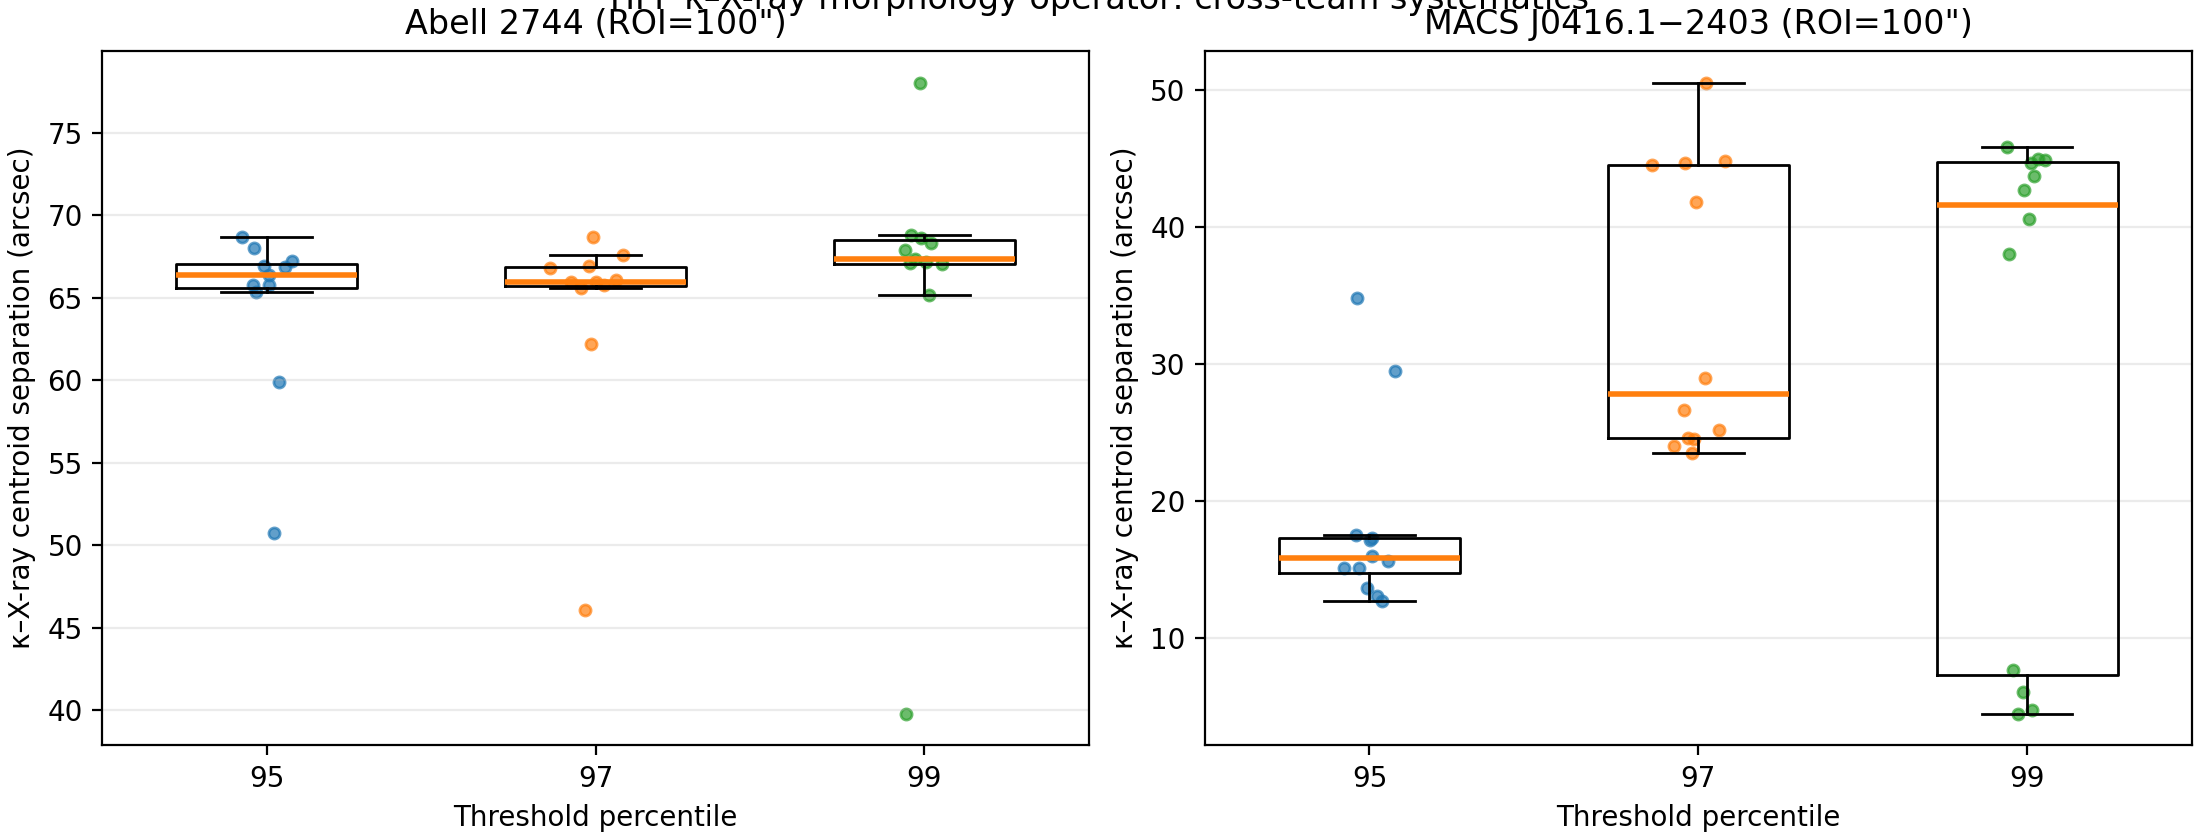
\includegraphics[width=\linewidth]{figures/hff_systematics_summary_roi100.png}
	\caption{HFF $\kappa$--X-ray systematics summary at ROI $=100^{\prime\prime}$ for Abell 2744 and MACS J0416.1$-$2403, showing cross-team dispersion under the fixed morphology operator across intensity thresholds.}
	\label{fig:hff-systematics-summary-roi100}
\end{figure}

\subsection{Six-panel diagnostic figures (ROI = 100″)}

For interpretability, we generated per-team six-panel diagnostics at ROI $= 100^{\prime\prime}$, including $\kappa$, X-ray proxy, threshold masks, and centroid overlays. Representative examples are shown below; the complete figure sets are available from the author upon request.

\begin{figure}[t]
	\centering
	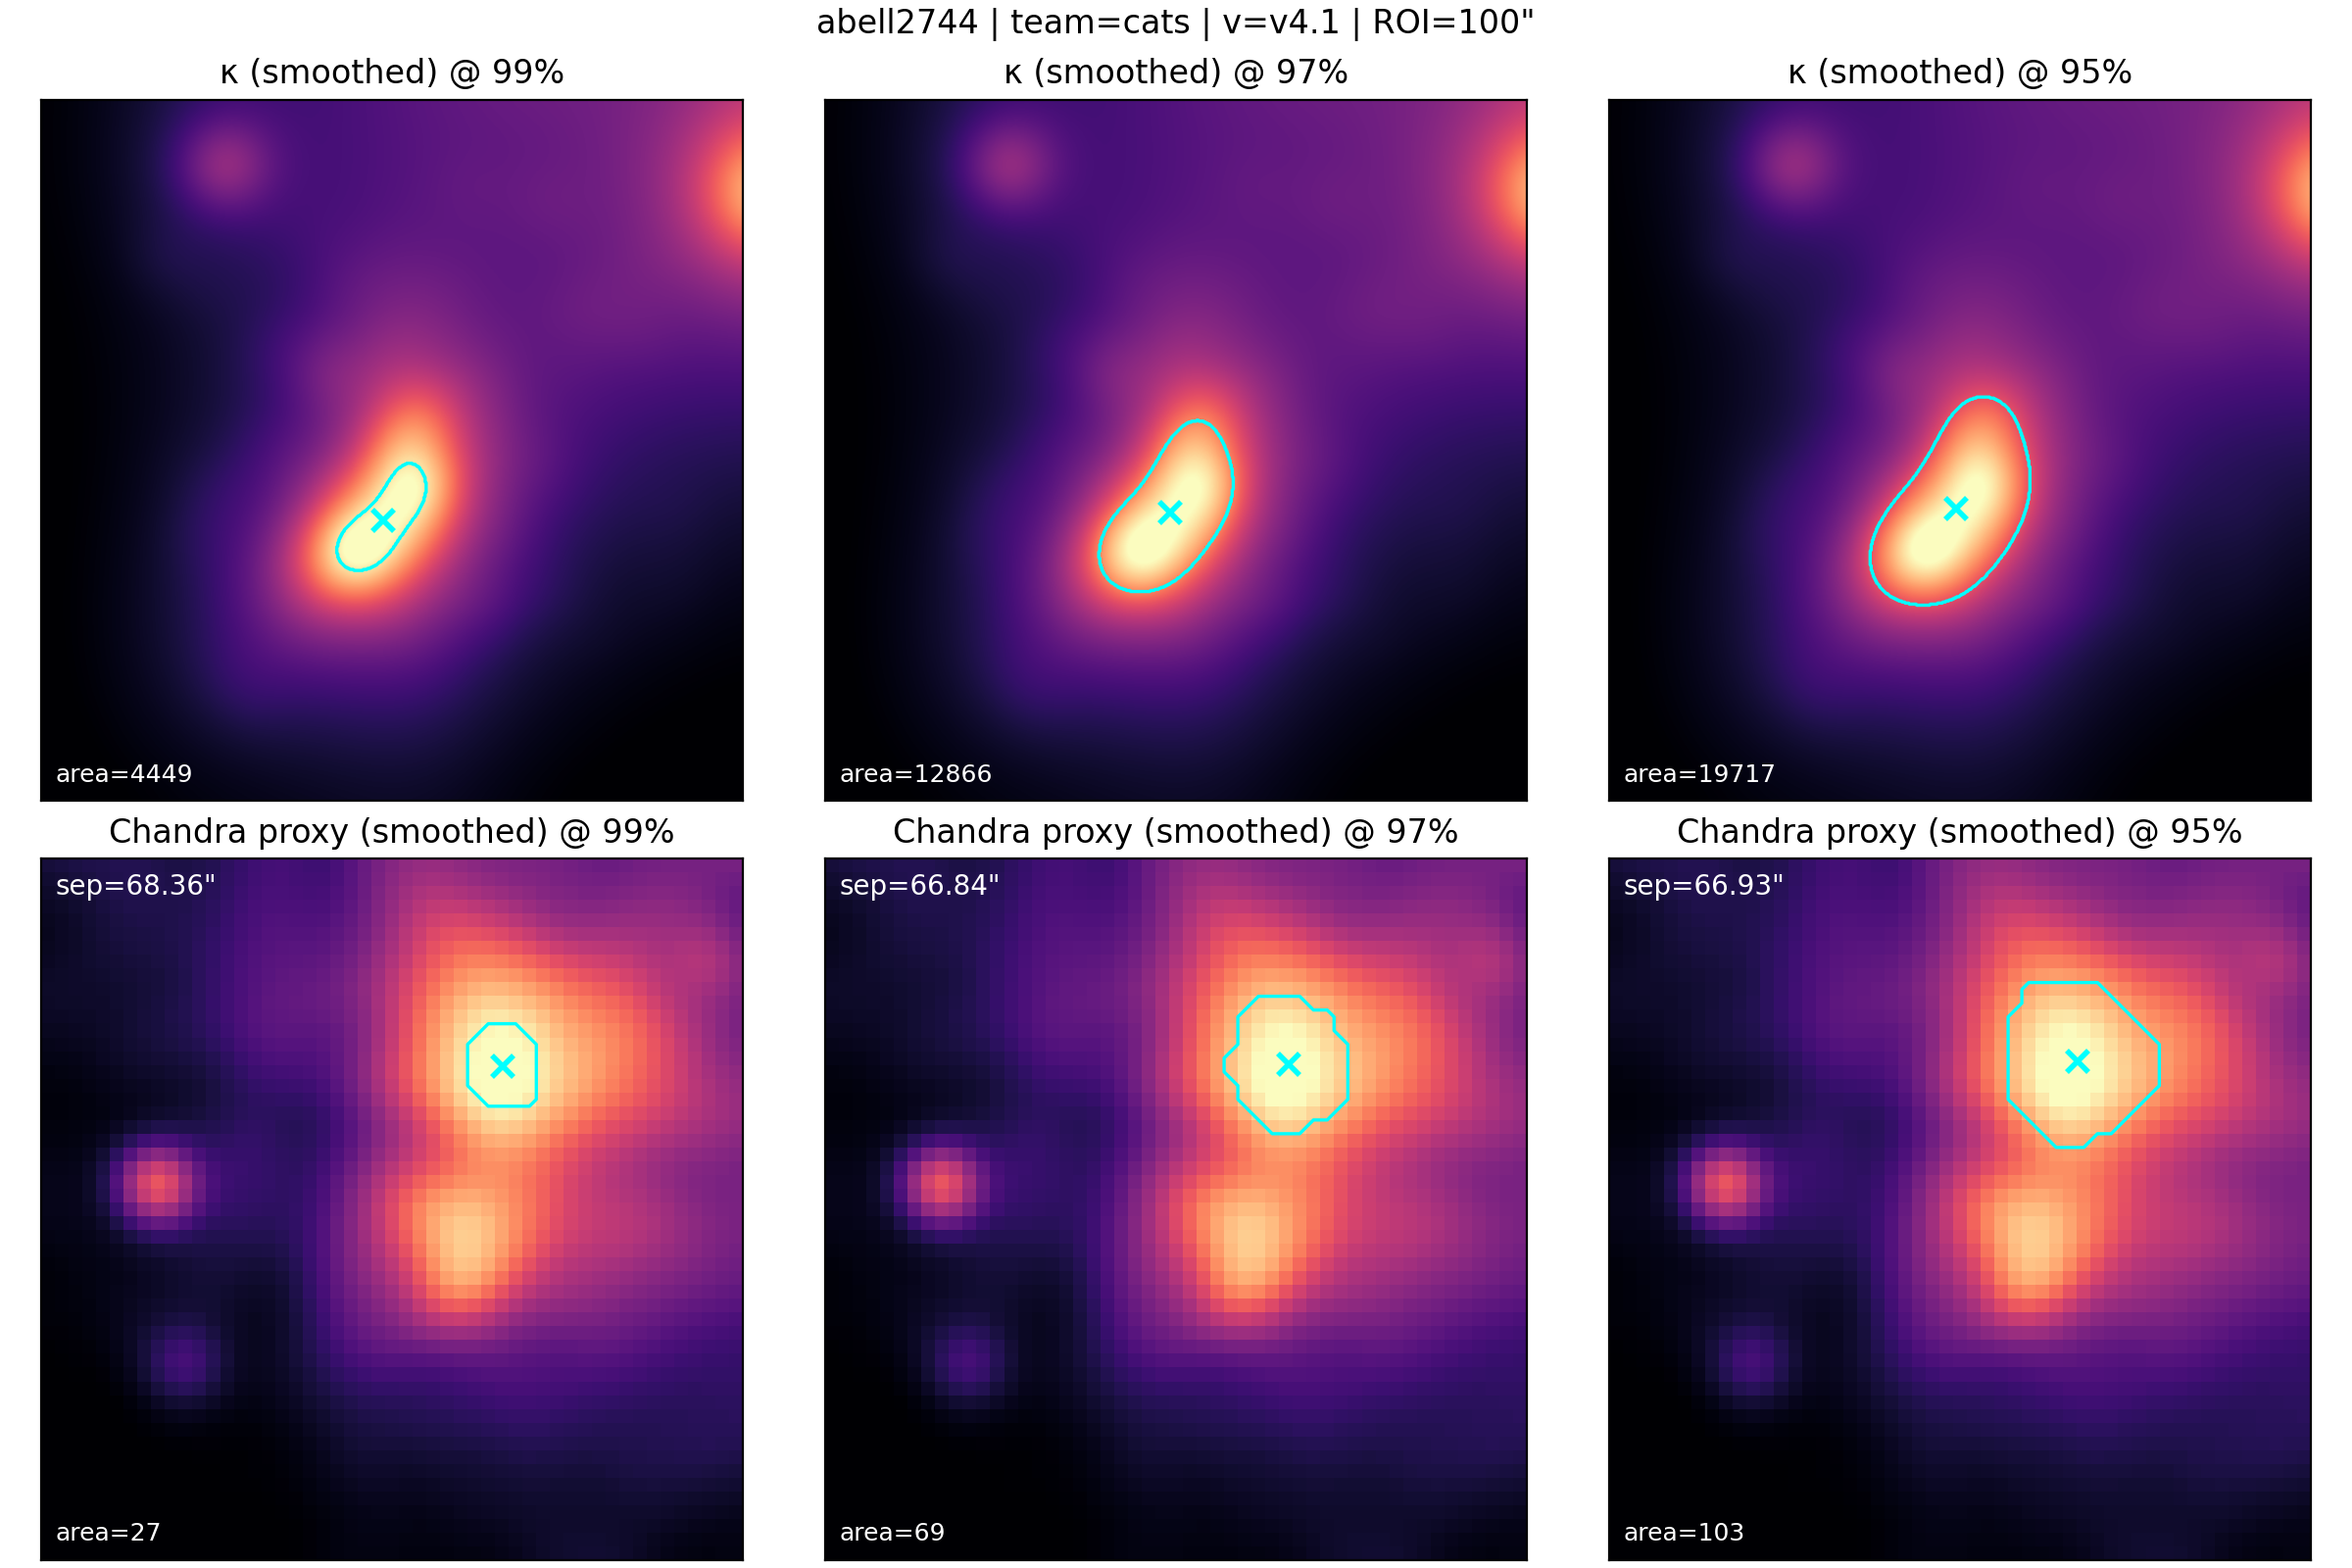
\includegraphics[width=\linewidth]{figures/abell2744_cats_v4p1_roi100_sixpanel.png}
	\caption{Six-panel diagnostic for Abell 2744 (CATS v4.1) at ROI $=100^{\prime\prime}$, illustrating the $\kappa$ field, X-ray proxy map, thresholded connected components, and centroid overlays used to compute the $\kappa$--X-ray separation.}
	\label{fig:abell2744-cats-v4p1-roi100-sixpanel}
\end{figure}

\begin{figure}[t]
	\centering
	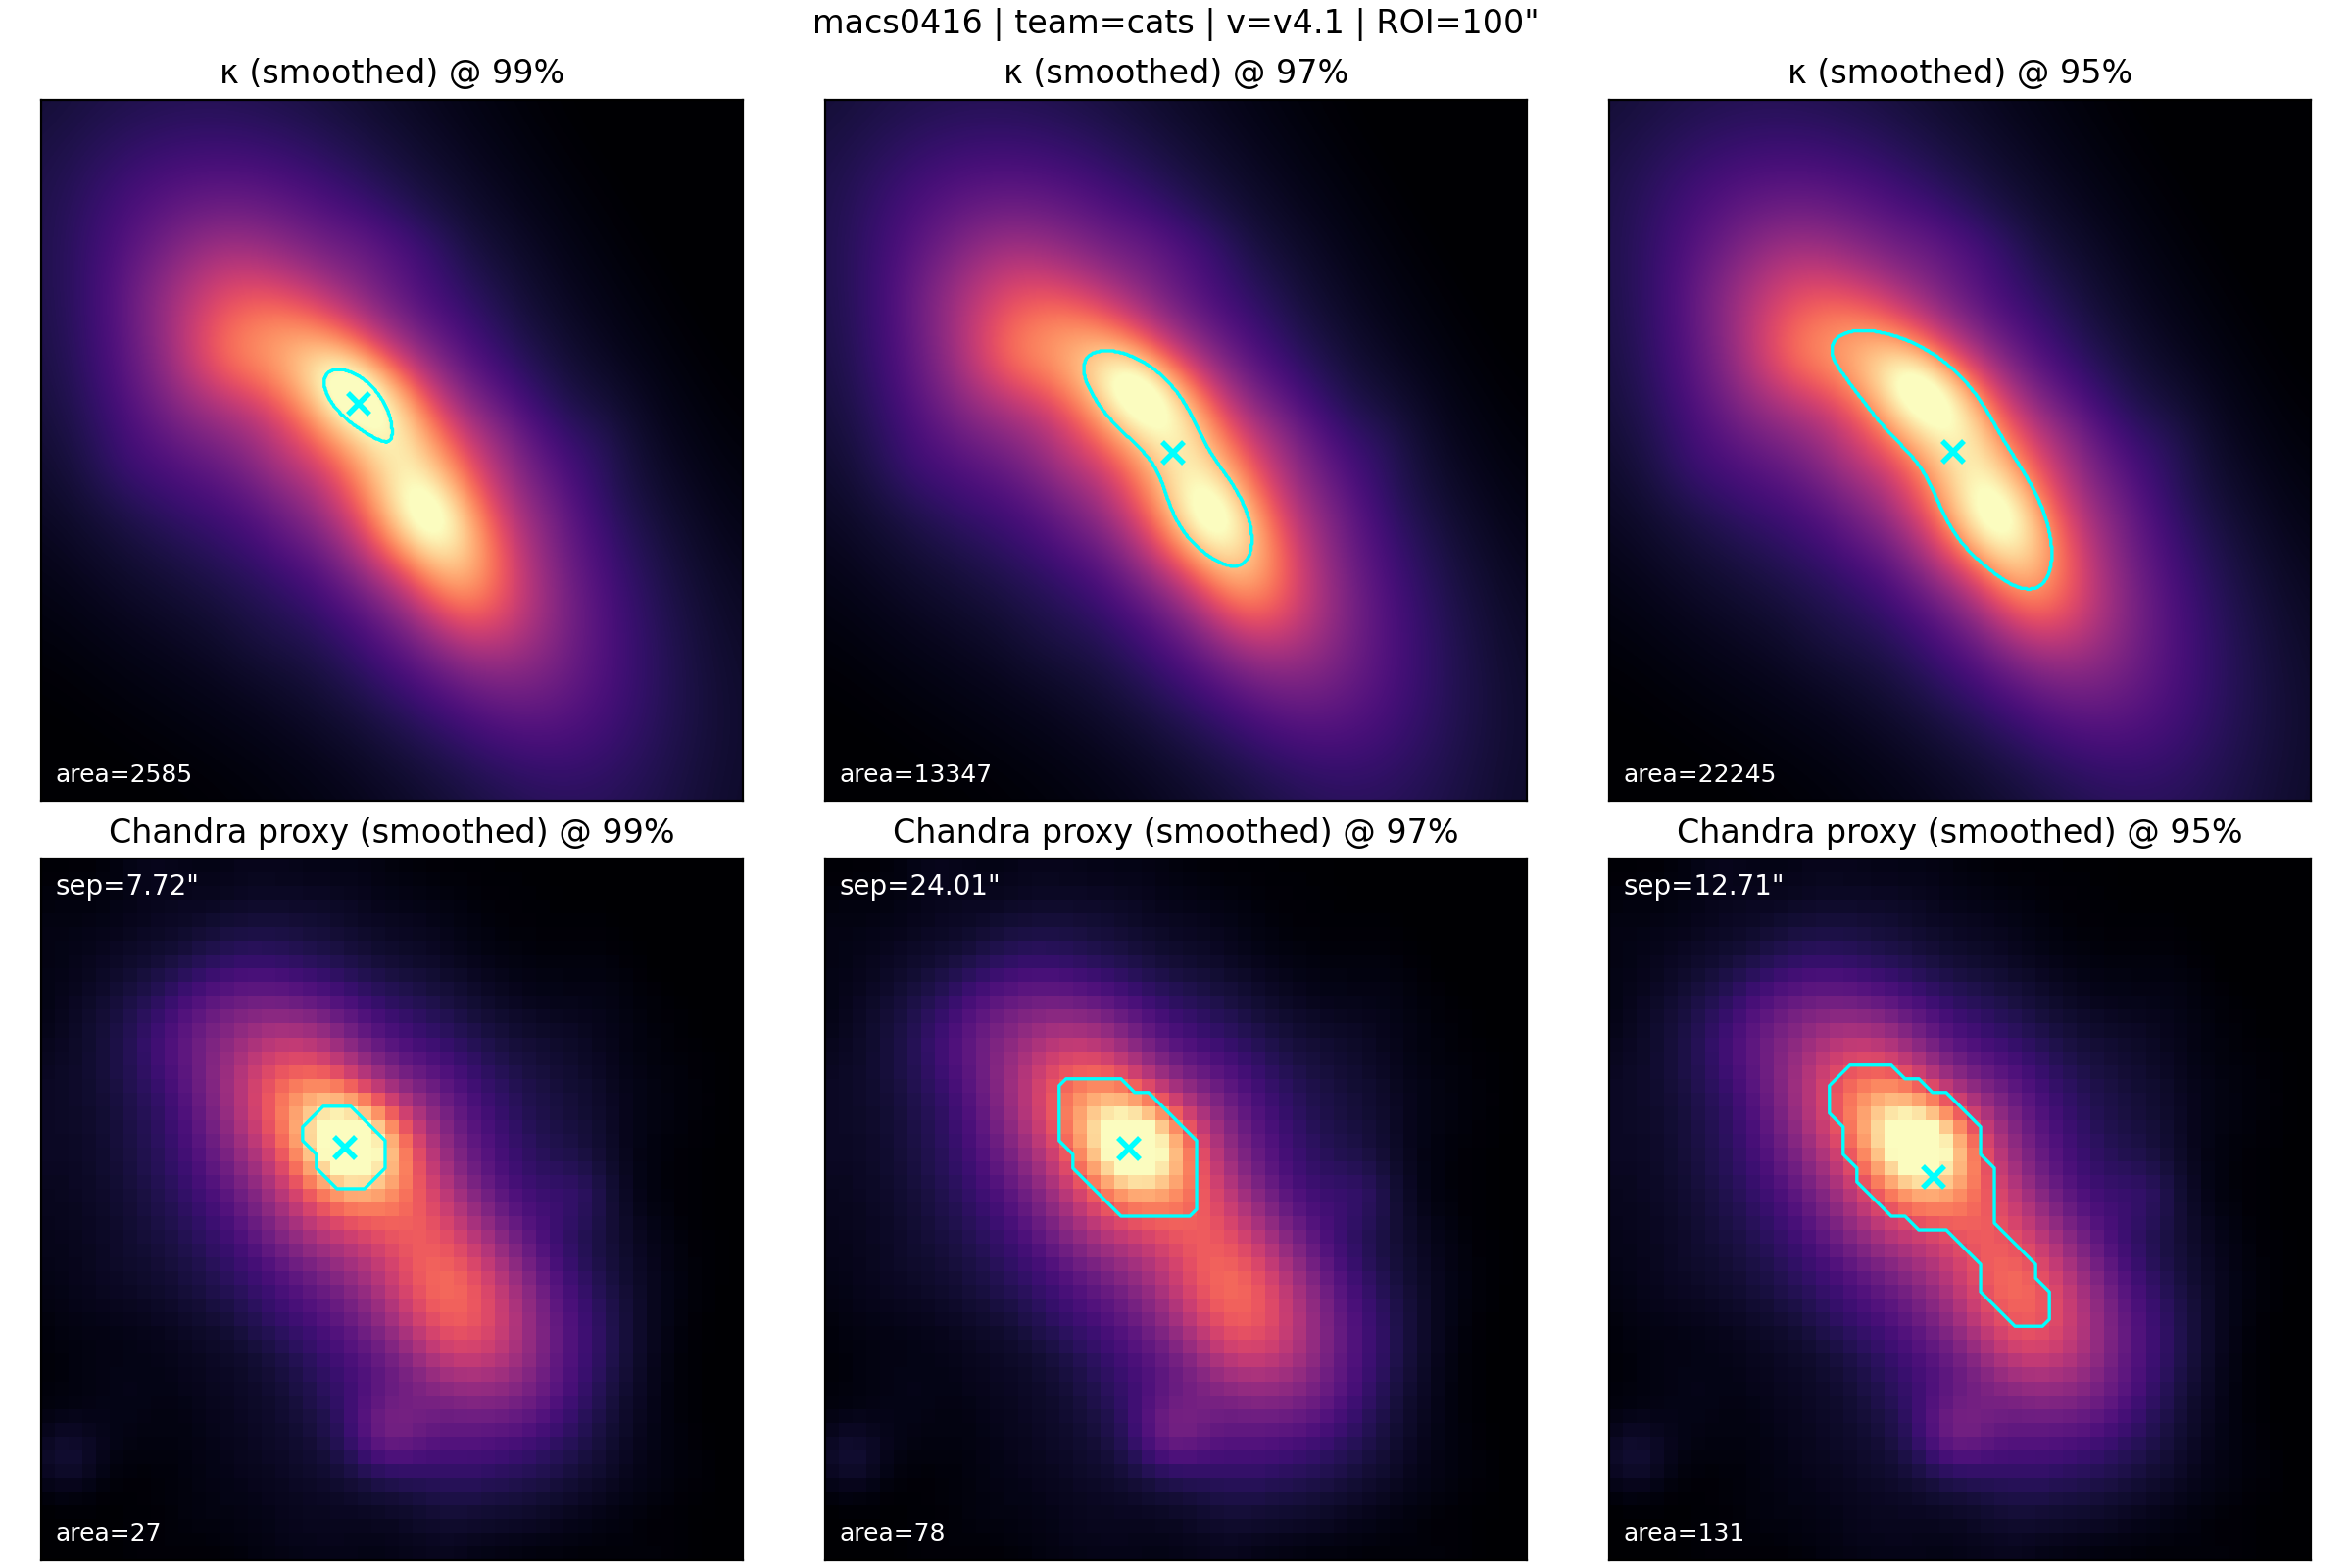
\includegraphics[width=\linewidth]{figures/macs0416_cats_v4p1_roi100_sixpanel.png}
	\caption{Six-panel diagnostic for MACS J0416.1$-$2403 (CATS v4.1) at ROI $=100^{\prime\prime}$, illustrating the $\kappa$ field, X-ray proxy map, thresholded connected components, and centroid overlays used to compute the $\kappa$--X-ray separation.}
	\label{fig:macs0416-cats-v4p1-roi100-sixpanel}
\end{figure}

\section{Appendix D. Spectral Harmonics and the Cymatic Analogy in Intrinsic Response Theory}

This appendix formalizes the ``cymatics'' analogy used throughout the paper by identifying a single spectral object---the eigen-spectrum of an intrinsic response operator---that plays the same mathematical role as Laplacian/biharmonic eigenmodes in Chladni plate experiments. In brief: eigenfunctions are the response-sector mode shapes, eigenvalues set the characteristic spatial scales, and nodal sets correspond to compression/rarefaction boundaries. Although the underlying response dynamics may be written covariantly on spacetime, the galaxy-rotation regime probed by SPARC is effectively stationary, so the empirically constrained ``harmonics'' are spatial overtones (additional radial nodes) rather than temporal frequency multiples.

\subsection{Purpose and scope}

The goal is to tie the qualitative ``pattern'' language to a concrete operator-theoretic object that can be constrained by the rotation-curve phenomenology.

\subsection{Unified operator statement (“DNA” of intrinsic response)}

Let \textbf{(see PDF; response-potential symbol not recovered)} denote the response-sector potential (or any equivalent scalar response field used to encode the inferred metric perturbation in the weak-field limit). Define the intrinsic response through a driven, self-adjoint elliptic operator on a spatial slice:

\textbf{(see PDF; driven elliptic operator equation not recovered from DOCX extraction)}

where \textbf{(see PDF; constitutive driving functional not recovered)} is the constitutive driving functional built from the baryonic sector, and the operator is taken in a minimal Sturm--Liouville form:

\textbf{(see PDF; Sturm--Liouville operator form not recovered from DOCX extraction)}

with \textbf{(see PDF; propagation coefficient not recovered)} controlling propagation (``permittivity/elasticity'') and $\beta(x)\ge 0$ encoding activation/screening (``mass'' or quenching). The intrinsic ``pattern DNA'' is the eigen-spectrum

\textbf{(see PDF; eigenproblem not recovered from DOCX extraction)}

yielding the modal response

\textbf{(see PDF; modal expansion not recovered from DOCX extraction)}

This is the direct analog of Chladni/cymatics: the eigenfunctions are mode shapes; eigenvalues set intrinsic spatial scales; and source overlap coefficients determine which modes are visible in a given galaxy.

\subsection{Where “harmonics” live in a unified spacetime theory}

In a unified spacetime theory, the fundamental response dynamics can be written covariantly (e.g., for a scalar template, a hyperbolic operator such as $\Box$ acting on a field). In stationary or quasi-stationary systems, variable separation reduces the covariant problem to a spatial eigenproblem: \textbf{(see PDF; separation-of-variables equations not recovered)}. SPARC rotation curves constrain the near-static regime in which the response has equilibrated, leaving the spatial spectral content as the observable imprint.

\subsection{Observable proxy: node count and Δ-sign flips in the SPARC window}

SPARC provides baryonic mass models and high-quality rotation curves for 175 disk galaxies. Define \textbf{(see PDF; residual definition and symbol not recovered)} operationally as the signed residual between the observed and baryonic expectations in the rotation curve (e.g., \textbf{see PDF; example residual expression}). In an oscillatory response sector, this residual (and therefore the inferred extra acceleration) can alternate in sign across radius, producing compression and rarefaction lobes. In the operator language above, each radial sign change corresponds to crossing a nodal annulus/shell of the net excited response pattern. Hence, within the finite SPARC radial sampling window, the number of sign flips provides a model-agnostic proxy for the degree of higher-(harmonic/overtone) participation: zero flips indicates a fundamental-dominated response; multiple flips indicate increasing harmonic content (higher node count) selected by the driving and by activation/quenching boundaries.

\subsection{Consequences for lensing and stability constraints}

Because the response tensor is inferred effectively from kinematics, sign-alternating lobes should be treated as an empirical prediction of the effective sector rather than as an immediate pathology. In particular, annular rarefaction phases imply a ring-like suppression of weak-lensing observables (e.g., \textbf{see PDF; observable symbols not recovered}) in the same radial ranges, providing a falsifiable discriminant using upcoming wide-field surveys. At the fundamental level, the minimal non-negotiable stability line is to keep the underlying response-field EFT free of ghosts/gradient instabilities; for broad $k$-essence classes this is ensured by requiring a positive kinetic coefficient \textbf{(see PDF; positivity/stability condition not recovered)}, which enforces the null energy condition for the fundamental field stress--energy even if the effective, inverse-constructed response density changes sign locally. For context, relativistic MOND completions (e.g., TeVeS) also introduce extra fields that alter lensing, but do not generically predict phase-correlated annular suppression tied to sign flips.



	\bibliographystyle{unsrtnat}
	\bibliography{references}
}

\end{document}
